% ---
% Capitulo Revisão de Literatura
% ---
\chapter{Revisão de Literatura}\label{chap:revisao-literatura}
% ---
\begin{citacao}
	\begin{flushright}  
\emph{``Todo enunciado - desde a breve réplica (monolexemática) até o romance ou o tratado científico - comporta um começo absoluto e um fim absoluto: antes de seu início, há os enunciados dos outros, depois de seu fim, há os enunciados-respostas dos outros [\ldots]. O locutor termina seu enunciado para passar a palavra ao outro ou para dar lugar à compreensão responsiva ativa do outro. O enunciado não é uma unidade convencional, mas uma unidade real, estritamente delimitada pela alternância dos sujeitos falantes'' (Bakhtin)}
	\end{flushright}
\end{citacao}

Este capítulo tem por objetivo clarificar conceitos considerando a evolução e as interesecções entre as concepções utilizadas, bem como dar um panorama geral de como as questões de gênero, de mobilidade e de sustentabilidade vêm sendo tratadas sob a perspectiva do planejamento de transportes. 
Buscou-se, sempre que possível, apresentar aspectos ligados à realidade brasileira e quiçá paulistana, pois o escopo espacial de análise do presente trabalho é a Região Metropolitana de São Paulo (RMSP) (ver Figura \ref{fig:mapa-rmsp}), área coberta pela Pesquisas Origem e Destino (Pesquisas OD) do Metrô-SP. 

\begin{figure}[htb]%
    \caption{\label{fig:mapa-rmsp}Mapa dos municípios que compõem a região metropolitana em 2014, divididos por sub-regiões \cite{LEI1139}}%
    \begin{center}%
        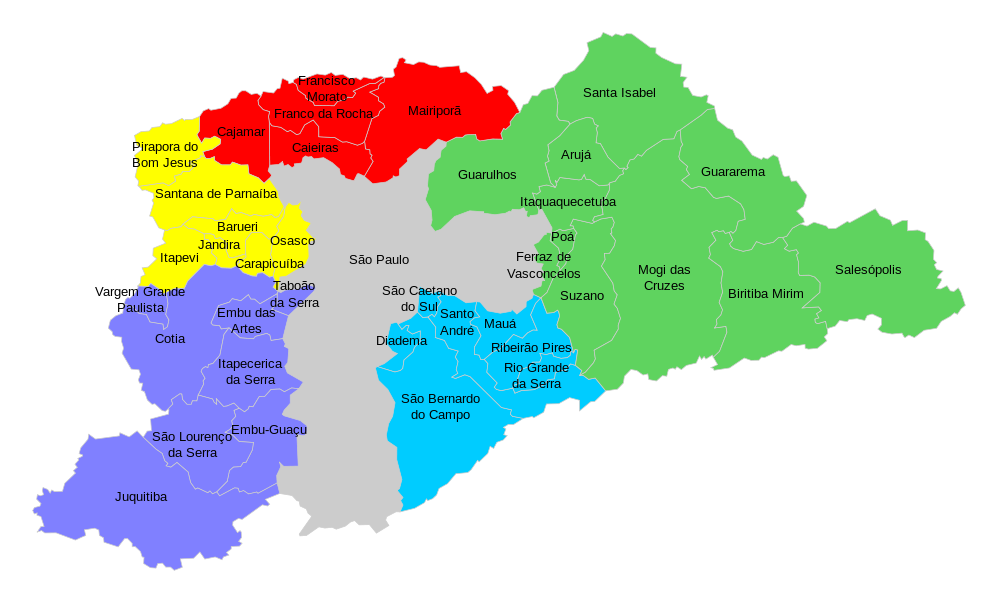
\includegraphics[width=0.9\textwidth]{./imagens/Mapa-RMSP-subregions.png}%
    \end{center}%
    \fonte{Mapa elaborado por Marcos Elias Oliveira Júnior, disponível em: \url{http://pt.wikipedia.org/wiki/Regi\%C3\%A3o_Metropolitana_de_S\%C3\%A3o_Paulo\#mediaviewer/File:Mapa-RMSP-subregions.svg} Acesso em 10 de novembro de 2014}
\end{figure}%

%Ao estudar o comportamento da mulher em relação ao do homem nos transportes são frequentes duas abordagens na literatura \cite{BEST2005}: a primeira considera principalmente as diferenças de gênero decorrentes do mercado de trabalho \cite{HANSON1985} e a segunda prioriza as diferenças decorrentes do medo feminino em resposta à violência masculina \cite{TRENCH1992}.
%O presente trabalho se aterá à primeira vertende de pesquisa, investigando indução de comportamentos tidos como femininos e como masculinos a partir de variáveis sócio-econômicas. Não serão considerados efeitos comportamentais decorrentes da violência, o que não significa dizer que tais aspectos sejam menos relevantes ou que não possam ser explorados em análises futuras.


\section{Gênero}
% META: 10p.

Ao nascer, umas das primeiras atividades do ser humano é comunicar-se, o que inclui nominar para si o mundo que o cerca. Esse processo não se dá de maneira solitária, a nominação advém de uma interação social que visa compartilhar signos afim de efetivar a comunicação. Por isso, este capítulo visa estabelecer o que se deseja exprimir através de palavras-chave deste trabalho (gênero, mobilidade e sustentabilidade), considerando a visão de Bakthin, cujo trabalho, segundo \citeauthoronline{STELLA2005} (\citeyear{STELLA2005}), indicava ser necessário

\begin{citacao}
não somente a palavra, mas também a linguagem em geral, ser concebida e tratada de uma outra forma, levando-se em conta sua história, sua historicidade, ou seja, especialmente a linguagem em uso. Isso significa que, no pensamento bakthiniano, a palavra reposiciona-se em relação às concepções tradicionais, passando a ser encarada como um elemento concreto de feitura lógica.
\end{citacao}

Há um senso comum que confunde e funde, não por acaso, os conceitos de sexo e gênero, muito embora sejam distintos - distinção esta encontrada em maior ou menor grau de acordo com o idioma. Em inglês a palavra \emph{sex} tem sentido mais limitado, ligado à anatomia, e a palavra \emph{gender} tem sentido mais amplo, ligado à construção cultural da identidade. Em francês, a palavra \emph{séxe} e, em alemão, a palavra \emph{Geschlecht}, designam tanto diferenças físicas como psicológicas, sociais e culturais \cite{FRAISSE2001}. \citeauthoronline{MORAES1998} (\citeyear{MORAES1998}) reporta que, em francês, frequentemente utiliza-se \emph{rapports sociaux de séxe} ao invés de \emph{gendre} para se designar \emph{gênero}. Comparado com o termo inglês \emph{gender}, ``a palavra gênero, em português, é um substantivo masculino que designa uma classe que se divide em outras, que são chamadas espécies'', definição então retirada do Novo Dicionário Aurélio por \citeauthoronline{MORAES1998} (\citeyear{MORAES1998}, p.101).
Já hoje, em 2014, o Dicionário Aurélio
\footnote{Dicionário Aurélio Online: \url{http://www.dicionariodoaurelio.com/genero} Acesso em 26 de setembro de 2014.}
já comporta entre suas definições, aquela em que \emph{gênero} pode ser entendido como o ``conjunto de propriedades atribuídas social e culturalmente em relação ao sexo dos indivíduos''.
Porém, entre as definições mais gerais apresentadas pelo Dicionário Michaelis, \emph{gênero} é definido da seguinte forma
\footnote{Dicionário Michaelis Online: \url{http://michaelis.uol.com.br/moderno/portugues/index.php?lingua=portugues-portugues&palavra=g\%EAnero} Acesso em 26 de setembro de 2014}:

\begin{citacao}
s.m. (lat *\emph{generu}, por \emph{genus}) 1 Grupo de seres que têm iguais caracteres essenciais. 2 \emph{Lóg.} A classe que tem mais extensão e portanto menor compreensão que a espécie. 3 \emph{Biol.} Grupo morfológico intermediário entre a família e a espécie. 4 \emph{Gram.} Flexão pela qual se exprime o sexo real ou imaginário dos seres. 5 \emph{Gram.} Forma do adjetivo ou pronome com relação ao gênero dos nomes a que se refere. 6 Agrupamento de indivíduos que possuem caracteres comuns. 7 Espécie, casta, raça, variedade, sorte, categoria, estilo etc. 8 Qualidade, espécie, modo.
\end{citacao}

Percebe-se que o termo gênero designa um conceito em construção e consolidação, não apenas no Brasil, sendo necessário defini-lo sempre que o utilizarmos como denominação de categoria de análise \cite{MORAES1998}. Para isso, será feito um breve apanhado do surgimento e trajetória da palavra \emph{gender} ou \emph{gênero} nas pesquisas acadêmicas, inclusive no Brasil, bem como a evolução do conceito.

O conceito fundido e identitário de sexo e gênero, como se fossem sinônimos, pertenece a uma visão binária de mundo que define as mulheres mais próximas das natureza, do trabalho reprodutivo, da passividade e do irracional e, em oposição, define os homens mas próximos à cultura, ao trabalho produtivo, à ação e à racionalidade \cite{HARAWAY2004}.
Estudiosas feministas, rejeitando o determinismo bio-sexual para a situação social das mulheres, precisavam desmontar a naturalização das diferenças entre homens e mulheres que vinculava suas relações sociais, políticas e econômicas a seu aparelho reprodutor \cite{PISCITELLI2009}. 
Para \citeauthoronline{HARAWAY2004} (\citeyear{HARAWAY2004}, p.218), as feministas lutaram ``para remover as mulheres da caegoria da natureza e colocá-las na cultura como sujeitos sociais na história, cosntruídas e auto-construtoras''. Desssa forma, a evolução do conceito de gênero mescla-se à história do feminismo.

A chamada ``primeira onda feminista'' ocorreu entre o final do século XIX e o início do século XX nos países hoje considerados desenvolvidos da Europa e da Américado Norte. A principal bandeira reivindicada direitos iguais, compondo uma ideia de que deveria haver uma igualdade entre os sexos. Em decorrência dessa primeira movimentação, em diversos países, as mulheres conquistaram alguns direitos equivalentes aos dos homens, como o voto. Essa conquista do voto como um direito político caracterizou o movimento sufragista, que não pode ser confundido com o movimento feminista, embora seja parte dele.
A Filândia foi o primeiro país a garantir direito a votar e ser votado(a) igualmente a mulheres e homens, em 1906, quando ainda era um Principado do Império Russo \cite{RAY1918}.
Na Inglaterra, em 1865, John Stuart Mill apresenta ao Parlamento um projeto de lei dando o voto às mulheres, que não foi aprovado. Somente em 1928, o voto feminino é autorizado nas mesmas condições àsdos homens \cite{NELSON2004}.
Nos Estados Unidos, foi em 1920 aprovada a 19ª Emenda
\footnote{Fonte: \url{http://www.archives.gov/historical-docs/document.html?doc=13&title.raw=19th+Amendment+to+the+U.S.+Constitution:+Women\%27s+Right+to+Vote} Acesso em 02 de novembro de 2014.} que proíbia o estabelecimento de qualquer restrição ao voto (estadual e federal) baseadas no sexo do(a) votante. 
 
No Brasil, o movimento sugfragista não teve tanta capilaridade nem foi um movimento de massas como nos Estados Unidos, Inglaterra ou Rússia. Ele teve início na década de 1910, quando o Partido Republicano Feminino é fundado no Rio de Jeneiro com o objetivo de instaurar o debate acerca do voto feminino. 
Bertha Lutz, filha do cientista Adolfo Lutz, licenciou-se em Ciências Naturais na Sorbonne de Paris e, ao retornar ao Brasil, funda a Federação Brasileira pelo Progresso Feminino, em 1919, que leva adiante a luta pelo sufrágio feminino \cite{PINSKY2003}. A primeira cidade a autorizar o voto feminino em eleições foi Mossoró (RN), em 1928. Em nível nacional, Getúlio Vargas autoriza o voto feminino apenas às mulheres solteiras, viúvas com renda própria ou casadas com a autorização do marido. A igualdade de condições de voto entre homens e mulheres se concretiza noa ano seguinte, 1932, pelo Decreto nº 21.076 que autoriza o voto a qualquer cidadã ou cidadão com idade superior a 21 anos.
A eleição de 1933 foi a primeira em que mulheres puderam participar do pleito, votando e sendo votadas, como Carlota Pereira Queiroz, a primeira deputada brasileira, que participou dos trabalhos na Assembleia Nacional constituinte entre 1934 e 1935 \cite{TABAK1989}.

Embora o direito ao voto tenha sido emblemático, a ideia de desfrutar de \emph{direitos iguais} na sociedade, mulheres e homens, tratava também de outros direitos como o acesso à educação e poder ter posse de bens - por muito tempo, de acordo com a lei, só homens podiam ser proprietários de casas, por exemplo \cite{PISCITELLI2009}. Subjacente aesses questionamentos das mulheres tecia-se o conceito de ``papel social'', bastante difundido a partir da década de 1930. Para \citeauthoronline{PISCITELLI2009} (\citeyear{PISCITELLI2009}, p.127), a teoria dos papeis sociais buscava:

\begin{citacao}
compreender os fatores que influenciam o comportamento humano. A ideia é que os indivíduos ocupam posições na sociedade, desempenhando papeis de filho, de estudante, de avô. [...] A ideia de posições ocupadas no desempenho dos papeis faz referência a categorias de pessoas qie são reconhecidas coletivamente. Um dos atributos que podem servir de base para a definição dessas categorias é a idade. [...] Outro desses atributos pode ser o sexo. Nesse caso, homens e mulheres desempenham papeis culturalmente cosntruídos: os papeis sexuais.
\end{citacao}

Ainda na década de 1930, Mead, uma antropóloga estadunidense, problematiza a fixitude dos conceitos \emph{feminilidade} e \emph{masculinidade} a partir de uma pesquisa comparativa entre três sociedades tribais na Nova Guiné  \cite{MEAD2000}. A pesquisadora conclui não haver um temperamento inato, universal que tenha origem biológica, ligada ao aparelho reprodutor. Ela observa que traços de caráter são aprendidos em sociedade, podendo, portanto, ser modificados e até desaprendidos. Ela deixa legado teórico que suporta a ideia de que existe uma cosntrução cultural da diferença sexual.
%http://pt.scribd.com/doc/178229042/Resumo-Sexo-e-Temperamento-Margareth-Mead

Em 1949, a filósofa francesa Beauvoir lança a obra \emph{O Segundo Sexo}, considerado precursor da ``segunda onda feminista''\cite{PISCITELLI2009}. Ainda que \citeauthoronline{BEAUVOIR1967} (\citeyear{BEAUVOIR1967}) não cite o conceito de  ``papel social'' ou mesmo ``papel sexual'', ela enfatiza logo de início que o conceito do que é ser uma mulher é uma construção social:

\begin{citacao}
nenhum destino biológico, psíquico, econômico define a forma que a fêmea humana assume no seio da sociedade; é o conjunto da civilização que elabora esse produto intermediário entre o macho e o castrado que qualificam de feminino.
\cite[p.09]{BEAUVOIR1967}
\end{citacao}

Em sua obra, \citeauthoronline{BEAUVOIR1967} (\citeyear{BEAUVOIR1967}) tem por foco questionar a dominação masculina, sem deixar de questionar também a eficácia do movimento feminista forjado até então no combate a essa dominação. Ela julgava ser possível esse combate ser bem sucedido ser fossem combatidos elementos como: forma com que mulheres eram educadas; instituição de casamentos opressores; maternidade compulsória; vigência de um duplo padrão de moralidade sexual que permitiam maior liberade sexual somente aos homens; e falta de trabalhos dignos e bem remunerados que possibilitassem independência econômica às mulheres. 

Quase que concomitantemente, nos Estados Unidos, nasce um novo par de categorias de estudos, o sexo-gênero \cite{FRAISSE2001,STOLKE2004,HARAWAY2004}. A distinção entre as característica biológicas e as características sociais torna-se mais difundida, ou seja, na academia e na sociedade passa ser ser considerada a noção de que posturas sociais de identidade masculina ou feminina não estabelecem relação biunívoca com o sexo anatômico.
A nominação dessa construção cultural pela palavra gênero ocorre em 1958, na Califórnia, quando foi empreendida uma pesquisa acerca da identidade de gênero no \emph{California Gender Identity Center}. Os resultados foram apresentados pelo psicanalista Robert Stoller em 1963, no Congresso de Pscicanálise de Estocolmo. Essa mesma pesquisa embasou a elaboração do primeiro volume de \emph{Sex and Gender} de \citeauthoronline{STOLLER1968} (\citeyear{STOLLER1968}). Essa obra expôs o quanto a relação sexo e gênero não é automática, nem estrita, discorrendo ainda sobre casos em que a anatomia da genitália não seria compatível com a identidade masculina ou feminina da pessoa. Assim, Stoller formula um conceito de gênero ligado à cultura, enquanto o conceito de sexo permanece ligado à morfologia corporal.

Em 1970 e 1980, o debate sobre esse par de categorias (sexo-gênero) toma espaço na comunidade acadêmica estadunidense. A antropóloga \citeauthoronline{RUBIN1975} (\citeyear{RUBIN1975})  introduz a categoria gênero no debate sobre opressões sociais sofridas pelas mulheres por meio do seu ensaio \emph{The Traffic in Women: Notes on the 'Political Economy' of Sex}. Nessa obra, \citeauthoronline{RUBIN1975} faz uma análise marxista sobreposta ao sistema sexo-gênero da qual depreende que no sistema de trocas capitalista, os homens estabelecem-se como vendedores e as mulheres são estabelecidas como mercadorias para serem trocadas.
Rubin dialoga com Lévi-Strauss que aponta ser o casamento o dispositivo mais importante de aliança entre as famílias, inexistente senão fosse pelo \emph{tabu do incesto} \cite{STRAUSS2010}. Segundo \citeauthoronline{PISCITELLI2009} (\citeyear{PISCITELLI2009}, para Rubin esse tabu é precedido por outro, o da \emph{homossexualidade}. Isso porque, mediante a divisão sexual do trabalho - tarefas atribuídas diferentemente de acordo com o sexo da pessoa - e ao tomar a menor unidade de sobrevivência econômica a família, tem-se necessariamente um homem e uma mulher, numa relação heterossexual de dependência mútua. Rubin discute também o trabalho doméstico, dando visibilidade a um trabalho que muitas vezes viabiliza o sustento do trabalhador (geralmente homem) sem que seja remunerada (a mulher). Por fim, ela consegue articular teoricamente gênero e sexualidade de forma que o conceito de gênero constituído até então não reside apenas em identificação com um determinado sexo, mas pressupõe que o desejo sexual seja por indivíduo do sexo oposto. 
% \url{https://ensaiosdegenero.wordpress.com/tag/gayle-rubin/} 
% \url{http://ensaiosdegenero.wordpress.com/2012/04/16/o-conceito-de-genero-por-gayle-rubin-o-sistema-sexogenero/}

A distinção entre sexo e gênero foi extremamente útil às feministas acadêmicas, pois sinalizava um lastro teórico para embasar os estudos sobre a condição da mulher, muitas vezes inferiorizada por sua condição biológica inerente. Com isso, o questionamento à lógica binária de interpretação do mundo passou a ser menos frequente e incisivo \citeauthoronline{HARAWAY2004} (\citeyear{HARAWAY2004}, p.218) e, porque não, superada em alguma medida. Conforme pode-se ver no trabalho de Rubin, o conceito de gênero foi além de separar dimensões culturais e biológicas de mulheres e homens. Cada vez mais o conceito de gênero passa a significar também a superação da leitura binária de mundo que só permite feminilidade ou masculinidade. Para \citeauthoronline{HEILBORN1992} (\citeyear{HEILBORN1992}, p.41):

\begin{citacao}
A categoria de gênero não deve ser acionada como um substituto de referência para homem ou mulher. Seu uso designa, ou deveria fazê-lo, a dimensão inerente de uma escolha cultural e de conteúdo relacional. Por outro lado, traz embutida a articulação desse código, que se apropria da articulação da diferença sexual tematizando-a em masculino e feminino, com outros níveis de significação dos universos.
\end{citacao}

Se a primeira onda do feminismo reinvindicou direitos iguais, a segunda onda avançou e lutou pelo exercícioigual dos direitos. Na primeira onda buscava-se provar que as diferenças entre o feminino e o masculino eram de origem social e não biológica. Tal afirmação não é abandonada na segunda onda, mas aprofundada, passando-se a buscar as origens de tais diferenças sócio-culturais. Nessa construção, segundo \citeauthoronline{PISCITELLI2009} (\citeyear{PISCITELLI2009}, p.133-134):

\begin{citacao}
A categoria ``mulher'' foi desenvolvida pelo feminismo da segunda onda em leituras segundo as quais a opressão das mulheres está além de questões de classe e raça, atingindo todas mulheres, inclusive as mulheres das classes altas e brancas. [...] O reconhecimento político das mulheres como coletividade ancora-se na ideia de que o que une as mulheres ultrapassa em muito as diferenças entre elas. Isso criava uma ``identidade'' entre elas.
\end{citacao}

Se essa uniformização entre as mulheres foi útil para forjar uma união na conquista por direitos, em meados da decada de 1970 e início dos anos 1980, já era questionada. Feministas negras e mulheres de países subdesenvolvidos \cite{FURTADO2009} cada vez menos identificavam-se com o arcabouço teórico hegemônico e homogêneo apresentado por feministas dos países do ``norte rico'', inclusive por Rubin. Assim, a ``terceira onda feminista'' desdobra-se em feminismos diversos. Afinal, as mulheres negras contam com um história diferente das mulheres brancas, grande parte das vezes tendo a escravidão e suas consequências como parte determinante da vida de sua ancestralidade \cite{HOOKS1990,CRENSHAW2002}. No caso de países subdesenvolvidos, como o Brasil, não cabe comparar \emph{ipsis literis} a trajetória das mulheres (mesmo brancas) brasileiras com as portuguesas, por exemplo. Segundo \citeauthoronline{PINTO2004} (\citeyear{PINTO2004}) as mulheres brasileiras são vistas como mais maternais, com vocação para a domesticidade e muito mais ``racializadas'' que as portuguesas.

%Mas, segundo \citeauthoronline{WIZEMAN2001}(\citeyearonline{WIZEMAN2001}) os termos sexo e gênero não são sinônimos e, conforme definição adotada pelo Instituto de Medicina da \emph{National Academy of Sciences} o sexo é uma classificação ``de acordo com os órgãos reprodutores e funções [biológicas] atribuídas pelo complemento cromossômico''. Gênero, por sua vez, é a ``auto-representação de um pessoa como masculino ou feminino, ou como a pessoa é percebida por instituições sociais com base na apresentação de gênero do indivíduo''.

%TODO
AQUI ENTRA SCOTT e 
\url{http://ensaiosdegenero.wordpress.com/2012/04/23/o-conceito-de-genero-por-joan-scott-genero-enquanto-categoria-de-analise/}

CAROL GILLIAN
Gilligan, Carol. In a different voice: psychological theory and women's development. Cambridge, Mass.: Harvard University Press, 1993. 184 pp

A partir dos anos 1990 o uso da categoria gênero tornou-se mais frequente no Brasil \cite{MORAES1998} e XXXXX

\citeauthoronline{MORAES1998}(\citeyear{MORAES1998}, p.100)
\begin{citacao}
A expressão relações de gênero, tal como vem sendo utilizada no campo das ciências sociais, designa, primordialmente, a perspectiva culturalista em que as categorias diferenciais de sexo não implicam o reconhecimento de uma essência masculina ou feminina, de caráter abstrato e universal, mas, diferentemente, apontam para a ordem cultural como modeladora de homens e mulheres. Em outra palavras, o que chamamos de homem e mulher não é o produto da sexualidade biológica, mas sim de relações sociais baseadas em distintas estruturas de poder.
\end{citacao}

\citeauthoronline{KEHL1998} (\citeyear{KEHL1998}), incorporando o trabalho de BLEICHMAR (1988), ao invés de apartar sexo de gênero, assinala que gênero é um conceito que inclui a dimensão biológica do sexo, não sem somar-lhe atributos que a cultura provê.

AQUI ENTRA BUTLER
\url{http://ensaiosdegenero.wordpress.com/2012/05/01/o-conceito-de-genero-por-judith-butler-a-questao-da-performatividade/}

Sob o ponto de vista de gênero e cidadania \citeauthoronline{BRITO2001} (\citeyear{BRITO2001}), a autora resgata o conceito de cidadania grego, que excluía mulheres e escravos, e pontua que ao longo da história as identidades de homens e mulheres foram construídas pressupondo uma dicotomia entre o âmbito público e o privado. A partir de 1970, pontua ela, com o movimento feminista passa a haver críticas e questionamentos quanto à natureza, à separação e à natural atribuição dessas esfera a um determinado sexo. Assim, elabora-se uma perspectiva de análise a partir do gênero, e não do sexo biológico, pois o conceito de gênero também compreende as dimensões social e política do termo. Ao invés de apenas questionar os pares conceituais sexo-gênero e/ou masculino-feminino no que diz respeito à atribuição do público e do privado, ela propõe que se reveja a definição do termo \emph{político}, sem considerar como natural a associação do público ao homem/masculino e do privado ao feminino. A autora analisa a atuação política feminina em diversos contextos históricos e cita como exemplo um estudo de \citeauthoronline{DUVERGER1955} (\citeyear{DUVERGER1955}) que detectou forte participação feminina no plano eleitoral, mas não no governamental.

AQUI ENTRA BLAY (Gênero e cidadania)

AQUI ENTRA BLAY (Gênero e trabalho)

AQUI ENTRA HIRATA (Gênero e trabalho)

AQUI ENTRA KERGOAT (divisão sexual do trabalho)


Although many more women are now entering the labour force than a few decades ago, they still have to undertake the larger share of household-related work.
\cite{BEST2005}


Fechar com um conceito (Scott, provavelmente) e fazer a ressalva:
Vale lembrar que o gênero concerne tanto a homens como mulheres, ainda que a maior parte das análises que se valham dessa categorias refiram-se às mulheres \cite{MORAES1998}








%divisão sexual do trabalho, da construção social dos papeis de gênero e principalmente do papel da mulher no mercado de trabalho.

%A ideia de divisão sexual do trabalho foi utilizada primeiro por etnólogos para descrever a divisão “complementar” das tarefas entre homens e mulheres nas sociedades que estudavam. Kergoat (2003) afirma que “a divisão sexual do trabalho é a forma de divisão do trabalho social decorrente das relações sociais de sexo; esta forma adaptada historicamente e a cada sociedade. Ela tem por características a destinação prioritária dos homens à esfera produtiva e das mulheres à esfera reprodutiva.” Além disso, expõe que essa forma de divisão pauta-se em dois princípios: o da separação e o da hierarquização. O princípio da separação explora a ideia de que há “trabalhos de mulheres” e “trabalhos de homens” enquanto o princípio da hierarquização explora a ideia de que o trabalho do homem (produtivo) vale mais que o da mulher (reprodutivo).

%A partir daí há um processo de legitimação naturalista, de que alguns autores discordam (Peyre et al., 1991), que empurra o gênero para o sexo biológico desenhando uma relação biunívoca entre papel social, o de gênero, e sexo biológico nato. É histórica a associação do feminimo à subejtividade, à reprodução, à irracionalidade e à natureza assim como do masculino à objetividade, à produção, à racionalidade e ao domínio da natureza. Shearer e Arrington (1993) apontam ainda que no discurso de filósofos como Bacon, Locke e Hobbes a natureza torna-se algo a ser conquistada e tranformada para propósitos humanos. A construção e papeis sociais diversos, separados e hierarquizados de acordo com o sexo, é que constitui a identidade de gênero. Logo, da mesma maneira como as outras formas de divisão do trabalho a sexual pode ser mudada visto que é uma construção social, função do espaço e do tempo. Por esta razão se denominará neste artigo a divisão do trabalho em função do gênero, e não em função do sexo.

%Na Suécia, um dos países com menor desigualdade de gênero do mundo, as estatísticas ainda apontam para um quadro de desequilíbrio: as profissões tidas tipicamente femininas como professora, enfermeira e assistente social oferecem pior remuneração à força de trabalho do que postos de trabalho tidos como masculinos, como de engenheiro ou de administrador de empresas. Ademais, em 1994, ainda na Suécia, as mulheres que trabalhavam período integral no setor privado ganhavam cerca de 78\% do que seus pares homens; no setor público esse valor subia para 83\%. Mesmo quando o recorte inclui apenas os estratos das pessoas com ensino superior, as mulheres não chegam a ganhar 90\% do que os homens exercendo mesma função e com mesmo tempo de carreira. Neste caso, observam-se os dois princípios, o da separação e o da hierarquização (Hamilton, 2001). De acordo com PNUD (2010) o Brasil apresenta 0,539 de Índice Gini, que expressa desiguldade de renda (0 corresponde à máxima igualdade e 1 à máxima desigualdade), ao passo que a Suécia apresenta 0,250. Sendo o Brasil é um país mais desigual que a Suécia espera-se, portanto, que as diferenças salariais tendam a ser ainda maiores.

%Houve um aumento enorme da participação feminina na força de trabalho assalariada, especialmente mulheres com filhos, no período pós-guerra. Nos EUA, em 1986, mais de 61\% das mulheres casadas e com filhos menores de idade trabalhavam fora de casa, ao passo que em 1960 essa marca era de apenas 27\%. Na Suécia também houve aumento da participação feminina, e o maior deu-se no setor de empregos de meio-período (Hamilton, 2001). No Brasil, no século XX, período pós-guerra, também se observou aumento do número de mulheres na PEA (população economicamente ativa) e a preferência por empregos que demandem menos tempo (até 20h ou de 20 a 40h). No período de 2001 a 2010, como é possível observar pela Tabela 1 houve declínio da porcentagem de mulheres nos trabalhos até 20h e manteve-se a preponderância da preferência por ocupações que demandem de 20 a 40h. Para homens, predomina historicamente uma jornada superior a 40h semanais.

%Embora a mulher tenha conquistado o direito de trabalhar fora de casa e, por conseguinte, receber remuneração própria, ela não deixou de ser responsável pelas tarefas domésticas. Assim, ela ampliou o leque de papéis sociais que desempenha, acumulando-os, constituindo a dupla jornada de trabalho. Isso molda seus interesses, suas atividades, seu padrão de viagens e também restringe significativamente suas reais possibilidades de empregos e também seu tempo livre, que poderia ser dedicado a atividades de lazer.

%"Scott apresenta urna importante contribuição ao debate ao propor o uso do gênero como categoria de análise a partir de uma definição abrangente pela qual é possível compreender a relações entre gêneros e a constituição da sociedade, onde se inclui necessariamente a dimensão política."

As mulheres no Brasil escravocrata dispunham de uma grande imobilidade geográfica e mesmo as mulheres das classes dominantes raramente saíam às ruas e, quando o faziam, nunca estavam desacompanhadas \cite{SAFIOTTI1976}.
Ao longo do tempo, a urbanização e a industrialização levaram à ampliação da classe média e ao crescimento do consumo. As mulheres entraram também neste processo, embora a maior parte da força produtiva feminina tenha sido absorvida, ao menos inicialmente, no setor de serviços e com enorme
concentração nos empregos domésticos, com menor rendimento.
No Brasil, no século XX, observou-se aumento de mulheres na população economicamente ativa e a preferência por empregos de jornadas
menores.

Ainda no século XXI, em estudo da Fundação Perseu Abramo (2010), observa-se que de 2001 a 2010 manteve-se a preponderância feminina em ocupações que demandam de 20 a 40h semanais.
Para homens, manteve-se o predomínio histórico de jornada superior a 40h semanais. O ingresso das mulheres no mercado de trabalho não alterou drasticamente o papel delas na família e, portanto, nas atividades ligadas às
tarefas domésticas.
Quando existe a posse do automóvel este fica mais frequentemente à disposição dos homens do que das mulheres.
As mulheres ao andarem de automóvel são, com maior frequência, passageiras, remetendo à ideia de “não andar desacompanhada fora de casa”. \citeauthoronline{FOX1983}(\citeyear{FOX1983}) já indicava os padrões de viagens das mulheres: elas fazem menos viagens, viagens mais curtas e rápidas. Além disso, usam menos o automóvel e mais o transporte público.

\clearpage
\section{Mobilidade Urbana}
% META: 10p.

%TODO
AQUI ENTRA página sobre definição de mobilidade de modo geral e fechamento no tema da mobilidade urbana.

``o estudo dos problemas urbanos é indissociável da relação campo-cidade. Por isso, o ofoc da an[alise, independente da época estudada, precisa abranger essa relação.'' \cite[p.154]{FREITAG2007}

A mobilidade urbana é um elemento fundamental para que seja possível garantir aos habitantes acesso aos bens que orferece \cite{IEMA2010}.

FALAR DE ACESSIBILDIADE e sua diferença de MOBILIDADE

\clearpage
\section{Sustentabilidades}
% META: 10p.

Por definição de sustentabilidade encontram-se nos dicionários descrições bastante simples e amplas, que podem ser resumidas como ``a qualidade de ser sustentável'' \cite{MICHAELIS2014}, o que posterga a dúvida para a questão: o que é ser sustentável? Segundo \citeauthoronline{BLACK2010} (\citeyear{BLACK2010}), é aquilo que pode ser mantido ou que dure. É evidente que tal durabilidade não é eterna, mas por um determinado período. A ideia da permanência leva a crer que tal período seja longo, que relacione-se à perspectiva de longo prazo, mas de quão longo se trata, é uma indefinição, até hoje. Hoje, inclusive, é cada vez mais frequente o uso do termo sustentável como modificador ao invés de sustentabilidade como um conceito fechado em si. Aqui, exploraremos o desenvolvimento  sustentável e o transporte sustentável como as ``sustentabilidades'' de interesse.

As primeiras preocupações e dicotomizações entre desenvolvimento e meio ambiente remontam o fim da década de 1960, com o Clube de Roma
\footnote{O Clube de Roma fora fundado em 1968 por Aurelio Peccei e Alexander King e que consistia num grupo de pessoas ilustres (empresários, líderes religiosos, políticos, entre outros) que se reuniam para discutir assuntos ligados à política, economia e, também, meio ambiente. Para saber mais: \url{http://www.clubofrome.org/} Acesso em 06 de novembro de 2014.}, que será o berço da obra \emph{The Limits to Growth}. Este livro, publicado em 1972, problematiza pela primeira vez a questão do crescimento exponencial \emph{versus} a finitude dos recursos disponíveis e também se propõe a simular e tentar prever as consequências da intereção antrópica com sistemas não-antrópicos \cite{MEADOWS1972}. Nesse mesmo ano, ocorre a Conferência sobre o Ambiente Humano das Nações Unidas em Estocolmo.

Em 1983, as Nações Unidas (ONU) fundam a Comissão Mundial sobre Meio Ambiente e Desenvolvimento (WCED), composta por 19 delegados de 18 países, com a missão de produzirem um estudo sobre desenvolvimento em escala global, considerando aspectos como sustentabilidade e meio ambiente num perspectiva de longo prazo. Assim, a expressão ``desenvolvimento sustentável'' aparece pela primeira vez em \citeyear{WCED1987}, no relatório \emph{Our Common Future} da WCED, também conhecido como \emph{Brundtland Report} 
\footnote{Gro Harlem Brundtland era o Primeiro Ministro da Noruega e foi quem comandou a Comissão Mundial sobre Meio Ambiente e Desenvolvimento (WCED). Fonte: \url{http://www.un-documents.net/our-common-future.pdf} Acesso em 06 de novembro de 2014.}, onde é apresentado o clássico conceito:

\begin{citacao}
desenvolvimento sustentável é aquele que satisfaz as necessidades do presente sem comprometer a capacidade das gerações futuras satisfazerem as suas próprias necessidades. Este conceito contém em si outros dois conceitos-chave: o de ``necessidades'', em particular as necessidades essenciais dos pobres do mundo, às quais deve ser dada prioridade absoluta; e a ideia de limitações impostas pelo estágio tecnologico e de organização social sobre a capacidade do meio ambiente de satisfazer as necessidades presentes e futuras. 
\cite[p.41]{WCED1987}
\end{citacao}   

Essa definição consolidou-se na Conferência das Nações Unidas sobre Meio Ambiente e Desenvolvimento ocorrida em 1992 no Rio de Janeiro, também conhecida como ECO-92. Em quase vinte anos, o conceito popularizou-se, ganhou robustez e também ficaram mais nítidas suas limitações de implementação. Um relatório de balanço da ONU publicado em 2010 \cite{ONU2010} indica haver convergência conceitual de que o desenvolvimento sustentável está alicerçado sobre três pilares: desenvolvimento econômico, equidade social e proteção ambiental. O mesmo documento reconhece, porém, que apesar de visionário e integrador, o conceito tem se mostrado de difícil implementação pelos países e pouco tem sido abraçado em sua completude pelas políticas das diversas nações. 

Embora o desenvolvimento sustentável pretenda englobar os três pilares, o desenvolvimento é frequentemente sinônimo de desenvolvimento econômico e a sustentabilidade fica muitas vezes compartimentada à questão ambiental \cite{ONU2010}. Um dos caminhos que vem sendo cosntruído para tentar superaressa dificuldade é tornar o conceito menos difuso e mais palpável por meio de indicadores \cite{CHAMBERS2000,BOULANGER2008,BARRETT2010,FORTES2012} e metas (de preferência quantitativas) a serem atingidas num determinado prazo \cite{ONU2010,ONU2014}.

Outra saída, não excludente com esta recém apresentada, é adicionar outros pilares na conceituação do que seja desenvolvimento sustentável, como faz 
\citeauthoronline{BANISTER2005} (\citeyear{BANISTER2005}). Ele elenca outros dois fatores como fundamentais: (i) participação e (ii) governança. A dimensão da participação refere-se a envolver todas pessoas interessadas e envolvidas no processo, a saber, indivíduos, empresas, indústrias e governos. Argumenta que criar excluídos do processo torna muito mais difícil desenvolver as estratégias necessária de mudança. A dimensão da governança incide diretamente no processo de tomada de decisão, logo, significa mudanças nas estruturas organizacionais para que sejam facilitadas decisões intersetoriais.

\citeauthoronline{BANISTER2005} (\citeyear{BANISTER2005}) destaca cinco lições aprendidas desde o \emph{Brundtland Report} a partir das experiências de sucessos e fracassos: (i) as reduções devem começar modestamente; (ii) desestímulo às emissões de dióxido de carbono (CO$_2$) deve contar com mecanismos fiscais; (iii) deve haver incentivos fortes em pesquisa e desenvolvimento em ciência e tecnologia na temática das mudanças climáticas; (iv) embora todos países devam contribuir para a diminuição de emissões de carbono, a liderança cabe às nações mais ricas; (v) é preciso ação imediata e incerteza não é uma boa razão para inação ou atitudes fracas.
Ao se falar em sustentabilidades, fala-se necessariamente de mudanças de paradigma, profundas, e que podem até mesmo ser inatingíveis \cite{GLASBY2002}, embora possam ser perseguidas.

Do ponto de vista econômico, a obra \emph{Limits to Growth} fez escola e trouxe à baila a hipótese de que o crescimento econômico teria um teto, função dos recursos (naturais) disponíveis. Contudo, há estudiosos que se opõem a isso, como \citeauthoronline{KRUGMAN2014} (\citeyear{KRUGMAN2014}) em seu recente artigo \emph{Slow Steaming and the Supposed Limits to Growth}. O economista argumenta que é possível manter o crescimento econômico real (do PIB) e ainda assim reduzir a emissão de gases do efeito estufa. Para chegar a essa conclusão ele apresenta uma demonstração - bastante simplista - que considera o consumo de energia dos navios em função de suas velocidades e conclui ser possível manter um caudal econômico constante e, concomitantemente, diminuir o consumo de energia do sistema.

Entre as principais preocupações no âmbito ambiental estão a diminuição das reservas de petróleo, aquecimento global por conta da emissão de gases do efeito estufa, poluição (atmosférica, sonora e hídrica) e presença de chuva ácida. Diversos estudos indicam que exite correlação entre a ocorrência de diversos tipos de doenças (cardiorrespiratórias, câncer, entre outras) e a exposição alguns poluentes presentes na atmosfera \cite{WHO2000,WHO2006,BRUNEKREEF2012,MIRANDA2012}. Em São Paulo, \citeauthoronline{GOUVEIA2006} (\citeyear{GOUVEIA2006}) observaram associação estatisticamente significante entre o aumento no nível de poluentes na atmosfera e o aumento de hospitalizações por causas diversas, em todos grupos etários estudados. As emissões de CO$_2$, indicado como o principal gás responsável pelo efeito estufa, aumentaram cerca de 60\% e a parcela cuja origem são os sistemas de transporte também aumentou de 19,3\% para 28,9\% entre 1971 e 2001 \cite{BANISTER2005}.

Sob o prisma da equidade social, o acesso equânime a oportunidades de educação, trabalho, saúde e lazer é um dos pontos centrais. A equidade, associada à ideia do ``ser justo'', inevitavelmente referir-se-á à distribuição social de custos e benefícios , bem como em que grau essa distribuição é considerada adequada e que corrobore para a promoção da justiça \cite{LITMAN2006}. Aqui também o transporte tem papel estruturador já que pode ser o elemento que provê ou barra o acesso às oportunidades. \citeauthoronline{SANCHEZ2003} (\citeyear{SANCHEZ2003}) já apontava que equidade seria um dos temas estratégicos nas políticas de transportes. As megalópoles latino-americanas são, por vezes, cidades ``partidas'' \cite{VENTURA2001} entre a ``legal'' e a ``real'' \cite{ALVA1997}
\footnote{Estima-se que cerca de 40\% ou mais da população possui moradia em condição irregular \cite{FREITAG2007}.},
onde as vias de circulação frequentemente são cicatrizes no tecido urbano - por exemplo, em São Paulo, o ``Minhocão'' \cite{ABASCAL2010}, os monotrilhos \cite{ROLNIK2010} ou mesmo uma rua na favela de Paraisópolis (ver Figura \ref{fig:paraisopolis-morumbi}), em São Paulo.

Pode-se observar nos três pilares clássicos da sustentabilidade o papel relevante dos transportes. \citeauthoronline{VASCONCELLOS2012} (\citeyear{VASCONCELLOS2012}) aponta ainda que a energia gasta na mobilidade por habitante de uma cidade, ou seja, quanta energia os moradores de um município precisam para deslocar-se permite ter uma ideia do ``grau de sustentabilidade'' da mesma. Dessa maneira, cabe uma breve discussão sobre transporte sustentável.

\clearpage
\begin{figure}[htb]%
    \caption{\label{fig:paraisopolis-morumbi}Divisa da favela de Paraisópolis com o a parte nobre do bairro Morumbi em São Paulo}%
    \begin{center}%
        
\includegraphics[width=0.60\textwidth]{./imagens/morumbiparaisopolis.jpg}%
    \end{center}%
    \fonte{Tuca Vieira/Folha Imagens, disponível em: \url{http://www.scielo.br/scielo.php?script=sci_arttext&pid=S0103-49792010000200005} Acesso em 11 de novembro de 2014}
\end{figure}%

Para Black, um transporte sustentável seria aquele que atende às ``atuais necessidades de transporte e mobilidade não devem comprometer a capacidade das futuras gerações satisfazerem as suas próprias necessidades'' \cite[p.151]{BLACK1996}, e também que ``provê transporte e mobilidade com combustíveis renováveis, minimizando as emissões prejudiciais ao ambiente local e globalmente, e prevenindo fatalidades, lesões e congestionamentos desnecessários'' \cite[p.12]{BLACK2010}.

Banister (\citeyear{BANISTER2005,BANISTER2008}) aponta algumas medidas a serem perseguidas para que se possa alcançar um transporte sustentável:
\begin{compactitem}[]
\item (i) reduzir a necessidade de viajar;
\item (ii) encorajar a troca para modos de transporte coletivo ou não motorizado;
\item (iii) reduzir o comprimento das viagens;
\item (iv) incentivar a adoção de sistemas e tecnologias de transporte mais eficientes, tanto para carga quanto para passageiros;
\item (v) reduzir a utilização de carros e caminhões de carga nas áreas urbanas;
\item (vi) reduzir, na fonte, ruídos e emissões dos veículos,
\item (vii) incentivar a utilização mais eficiente e ambientalmente consciente do estoque de veículos;
\item (viii) melhorar a segurança de pedestres e de todos usuários das (rodo)vias;
\item (ix) melhorar a atratividade das cidades para seus moradores, trabalhadores, compradores e visitantes.
\end{compactitem}



\clearpage
\section{Intersecções e Sobreposições}
% META: 10p.

Nos últimos 20 anos o assunto gênero e transporte tem atraído atenção crescente da comunidade científica. Pesquisadores começaram a examinar os padrões de mobilidade com o recorte de gênero considerando que há acesso desigual a recursos materiais e diferenças na escolha modal. São comuns duas abordagens, a primeira que considera principalmente as diferenças de gênero decorrentes do mercado de trabalho (Hanson e Johnston, 1985) e a segunda que prioriza as diferenças decorrentes do medo feminino da violência masculina (Trench et al., 1992). O escopo deste trabalho se limita à primeira abordagem.

Embora a divisão de trabalho por gênero seja identificada como um fator que influencia a mobilidade, costuma-se ver o trabalho doméstico como uma restrição na participação do mercado de trabalho e o transporte decorrente desta atividade. Subestima-se o efeito do arranjo familiar no padrão de atividades femininas e as viagens geradas a partir de demandas domésticas. Se no mercado de trabalho vem sendo traçado um caminho que tende a diminuir o desequilíbrio de gênero, no trabalho doméstico ainda é a mulher a grande responsável pela sua execução.

A participação no mercado de trabalho aumenta o uso do carro para ambos os gêneros, especialmente quando se trata de meio-período. Ao diminuir entre homens e mulheres a diferença na participação no mercado de trabalho diminui-se também a diferença entre os rendimentos e espera-se que o padrão de viagens das mulheres passe a se assemelhar aos dos homens. Além disso, pode-se esperar que haja um aumento no uso do carro pelas mulheres devido à pressão para que deem conta tanto do trabalho formal como do trabalho doméstico pois se trata de um modo que confere flexibilidade de horário e de trajeto, bem como relativa rapidez. Entretanto a presença de criança na família gera o seguinte efeito: a maternidade reduz a probabilidade de o uso do carro por mulheres e a paternidade a aumenta para homens. (Best e Lanzendorf, 2005).


Labour force participation on the other hand, especially when part-time, intensifies car use for both genders. (BEST2005)
While parenthood reduces the odds of car use by women, it increases men’s car use. (BEST2005)

Women usually have shorter work-trips, use public transport more frequen- tly, and tend to trip-chain more often than men (Jones et al., 1983; Hjorthol, 2000; Rosenbloom, 1998; McGuckin and Murakami, 1999; Root and Schintler, 1999)

``os relatos dos cronistas, viajantes e historiadores do período nos exibem um quadro em que a menina ou a mulher [burgues] candidata ao casamento é extremamente bem cuidada, é trancafiada nas casas, etc.''\cite{DINCAO2012}

Ao analisar as viagens motivo trabalho há diferenças significativas indicadas por recentes pesquisas de países ocidentais. Neste tipo de viagem as mulheres costumam usar mais transporte público do que os homens e fazer mais cadeias de viagens, ou seja, usar uma combinação de diversos modos de transporte na consecução de uma viagem (Hjorthol, 2000).

Entende-se que o principal motivo dessas diferenças seja a desigual distribuição do trabalho doméstico, que leva a diferentes padrões de atividades e, assim, de viagens. Na Alemanha, por exemplo, a quantidade de tempo dispendida pelos homens com tarefas da casa se manteve constante nas últimas décadas, não tendo alteração significativa com o crescimento da participação feminina no mercado de trabalho (Künzler, 1994). O trabalho doméstico gera viagens, que Best e Lanzendorf denominam como viagens de “manutenção” do lar, isto é, aquelas relacionadas ao trabalho físico de emocional que reprodução da força de trabalho ou da sociedade em si. Novamente nota-se a mulher ligada a atividades de reprodução, apartada da esfera produtiva – princípio da separação. São atividades representativas para compor essa demanda de viagens de “manutenção”: compras, cuidados com as crianças (por exemplo, ir e voltar do pediatra, levar e trazer da escola) e cuidados com idosos (por exemplo, acompanhar ao médico).

Ter à disposição um carro para uso privado é o fator que mais influencia o seu uso em viagens motivo “manutenção”. Outros fatores que estimulam o uso do carro são: renda familiar e participação no mercado de trabalho. Se há mais renda familiar, há mais condições financeiras de adquirir um carro para tê-lo à disposição. Se há mais pessoas na família que fazem parte do mercado de trabalho, há mais interesse em comprar um carro, seja por aumento da renda familiar, seja pela necessidade de modo com flexibilidade de rota.

As grandes compras geralmente são feitas utilizando-se o carro, especialmente num contexto de padrão de consumo em que se expandem os grandes hipermercados, no Brasil, que precisam de grandes áreas urbanas e vendem em grandes volumes. Desta forma, estes empreendimentos têm localização menos central e buscam estar próximos de grandes avenidas. Essas condições de contorno (facilidade de acesso por carro e estímulo a grande volume de compras) tendem a levar o usuário a preferir o carro como meio de transporte.

Já as pequenas compras geralmente são feitas a pé e estas são majoritariamente feitas pelas mulheres. Trata-se da compra diária na padaria, na farmácia, no mercado do bairro, entre outras. Porém, no Brasil, as pesquisas Origem-Destino costumam ignorar as viagens feitas a pé num raio inferior a 500m, o que inclui grande parte das viagens de “manutenção” como as de pequenas compras de abastecimento doméstico (Metrô, 2007).

A presença de criança é um fator que impacta bastante no padrão de atividades da família, de forma diferentes para pais e para mães. Um estudo feito na Alemanha indica que mães usam menos frequentemente o carro do que mulheres sem filhos, ao passo que pais usam mais o carro do que homens sem filhos (Best e Lanzerndorf, 2005). Esse comportamento pode se dever ao fato de que os homens, antes da paternidade, já estão mais familiarizados com o uso do carro e tendem a não trocar sua escolha modal. Vale ressaltar que as escolas, em especial que atendem as crianças nas primeiras idades, geralmente ficam próximas à residência e que a maior parte das viagens para levar crianças à escola são a pé, feita pelas mães, que se estiverem num raio inferior a 500m, no Brasil, passam despercebidas.

Conflicting evidence exists in the literature on commuting about whether or not the greater household responsibilities of women lead to their widely observed shorter work trips compared to men. In light of changes in American household structures, this study reexamines the household responsibility hypothesis by focusing on household type (defined in terms of number of workers present in the home). Male and female work-trip distances are compared for Baltimore workers in single-worker households and for those in two-worker households. The findings support the household responsibility hypothesis by showing a larger and more significant sex disparity among respondents in two-worker households than among those in single-worker households even after controlling for other factors, including presence of children. These results, and the finding that married women have shorter work trips than married men, are in line with the general conclusions of some previous studies that the unequal division of labor within the household is partly responsible for the gender difference. \cite{IBIPO1992}


No Brasil, o olhar integrador entre transportes, planejamento urbano, meio ambiente e aspectos sociais tem sido cada vez mais frequente. Dois exemplos são o Estatuto da Cidade (\citeyear{ESTATUTOCIDADE}), obrigatório para cidade com mais de 20 mil habitantes, e o Plano Nacional de Mobilidade Urbana (\citeyear{PNMU}), obrigatório para cidades com mais de 500 mil habitantes. Tratam-se de dois instrumentos legais que norteiam elaboração de políticas públicas e, de acordo com \citeauthoronline{IEMA2010}(\citeyear{IEMA2010}):

\begin{citacao}
Estatuto da Cidade estabelece o direito às cidades sustentáveis para a atual e as futuras gerações, [sendo esse direito] compreendido como o acesso ao solo urbano, moradia, saneamento, infraestrturua, trabalho, lazer e serviços públicos.
\end{citacao}


\begin{citacao}
A descrição e análise dos fenômenos de megalopolização que ocorrem durante os últimos 500 anos surpreendem pela convergência de padrões na maioria das megalópoles latino-americanas aqui apresentadas. Eles não podem ser atribuídos à história, mas apontam para forças macroestruturais que promovem um desenvolvimento urbano que converge para a ``insustentabilidade'' das megalópoles na era da globalização. \cite{FREITAG2007}
\end{citacao}


